% \documentclass[12pt]{report}
% \usepackage{tikz}
% % 
\documentclass[tikz,border=5mm]{standalone}
% \usepackage[]{pgf}
% \usepackage[rgb]{xcolor}
\usepackage{pgfplots}

\usetikzlibrary{arrows,shapes,automata,backgrounds,petri,positioning}

\usetikzlibrary{arrows,calc}
\usetikzlibrary{decorations.markings}
\usetikzlibrary{arrows.meta}
\usetikzlibrary{fadings}

\usetikzlibrary{decorations.pathmorphing}
\usetikzlibrary{decorations.shapes}
\usetikzlibrary{decorations.text}
\usetikzlibrary{decorations.fractals}
\usetikzlibrary{decorations.footprints}
\usetikzlibrary{shadows}
\usetikzlibrary{calc}
\usetikzlibrary{spy}
\usetikzlibrary{intersections, pgfplots.fillbetween}

\tikzset{pfade/.style n args={3}{
    postaction={
    decorate,
    decoration={
    markings,
    mark=between positions 0 and \pgfdecoratedpathlength step 0.1pt with {
    \pgfmathsetmacro\myval{multiply(
        divide(
        \pgfkeysvalueof{/pgf/decoration/mark info/distance from start}, \pgfdecoratedpathlength
        ),
        100
    )};
    \pgfsetfillcolor{#3!\myval!#2};
    \pgfpathcircle{\pgfpointorigin}{#1};
    \pgfusepath{fill};}
}}}}



\pgfdeclaredecoration{complete sines}{initial}
{
    \state{initial}[
        width=+0pt,
        next state=sine,
        persistent precomputation={\pgfmathsetmacro\matchinglength{
            \pgfdecoratedinputsegmentlength / int(\pgfdecoratedinputsegmentlength/\pgfdecorationsegmentlength)}
            \setlength{\pgfdecorationsegmentlength}{\matchinglength pt}
        }] {}
    \state{sine}[width=\pgfdecorationsegmentlength]{
        \pgfpathsine{\pgfpoint{0.25\pgfdecorationsegmentlength}{0.5\pgfdecorationsegmentamplitude}}
        \pgfpathcosine{\pgfpoint{0.25\pgfdecorationsegmentlength}{-0.5\pgfdecorationsegmentamplitude}}
        \pgfpathsine{\pgfpoint{0.25\pgfdecorationsegmentlength}{-0.5\pgfdecorationsegmentamplitude}}
        \pgfpathcosine{\pgfpoint{0.25\pgfdecorationsegmentlength}{0.5\pgfdecorationsegmentamplitude}}
}
    \state{final}{}
}



\definecolor{counterjet}{HTML}{fbd9a8}
\definecolor{counterline}{HTML}{ff2b01}
\definecolor{counterbline}{HTML}{ff8a73}

\begin{document}
\begin{tikzpicture}[spy using outlines]
% \node(x0)  at (-0.33,0.1) {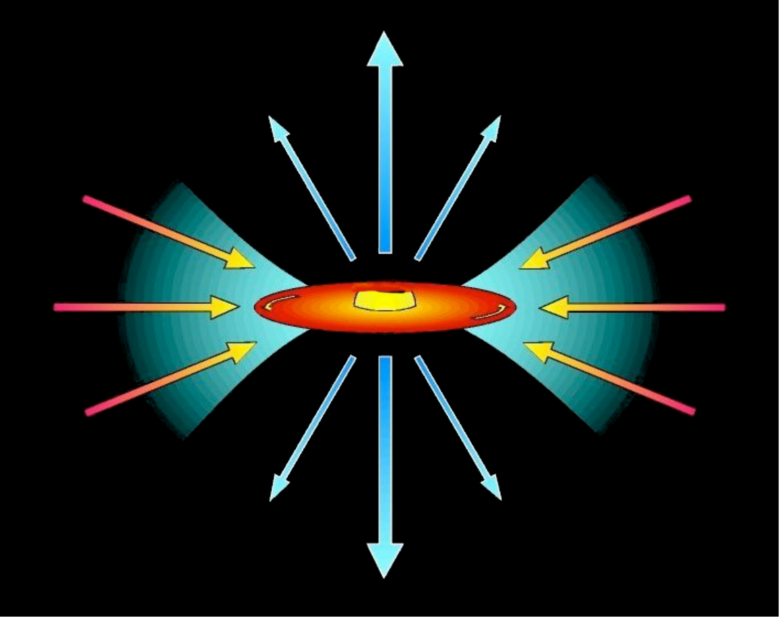
\includegraphics[height=8cm,width=12cm,angle=0,trim={3cm 2.5cm 3.5cm 2cm},clip]{../figs/ctts2.pdf}};

% \draw[help lines] (-10,-10) grid (13,10);


% \path[draw=red,use as bounding box] (-6,6) rectangle ++(#2);% remove 'draw=red' if you don't want a frame
% \clip (-5,-2.5) rectangle (5,6);

\def\left{(-2,0)      .. controls (-3,0.5) and (-4,0) ..    (-5,4) };
\def\right{(2,0)      .. controls (3,0.5) and (4,0) ..    (5,4) };
\def\up{(-5,4) -- (5,4)};
\def\bottom{(-2,0) -- (2,0)};

\draw[name path=A, yellow!2]   \left;
\draw[name path=B, yellow!2]    \bottom;
\draw[name path=C, yellow!2]   \right;
\draw[name path=D, yellow!2]    \up;

\tikzfillbetween[of=A and C]{opacity=1, yellow!40};
\tikzfillbetween[of=B and D]{opacity=1, yellow!40};
\draw[color=yellow,very thick,inner color=white, outer color=yellow!20,even odd rule] (0,4) ellipse (5.0 and 1);

\def\left{(-2,0)      .. controls (-1,-0.5) and (-3.5,0) ..    (-4.33,-2) };
\def\right{(2,0)      .. controls (1,-0.5) and (3.5,0) ..    (4.33,-2) };
\def\up{(-4.33,-2) -- (4.33,-2)};
\def\bottom{(-2,0) -- (2,0)};

\draw[name path=A, green!2]   \left;
\draw[name path=B, green!2]    \bottom;
\draw[name path=C, green!2]   \right;
\draw[name path=D, green!2]    \up;

\tikzfillbetween[of=A and C]{counterjet};
\tikzfillbetween[of=B and D]{counterjet};
% \draw[fill=yellow!15!orange, yellow!15!orange] (0,-2.5) ellipse (5.0 and 1);
\draw[color=counterbline,very thick,fill=counterjet] (0,-2) ellipse (4.31 and 0.7);

\begin{scope}[shift={(0,0)}]
\clip(-5,-3)rectangle(5,-2);
\draw[color=counterline,very thick,fill=counterjet] (0,-2) ellipse (4.315 and 0.7);
\end{scope}





\def\incurve{(0,0) ellipse (1.2 and 0.4)}
\def\outcurve{(0,0) ellipse (4 and 0.8)}

\def\ringin{(0,0) ellipse (2.2 and 0.55)}

\draw[fill=white]\ringin;
\def\ringout{(0,0) ellipse (2.4 and 0.64)}

% \def\incurve{(0,0) ellipse (1.2 and 0.4)}
% \def\outcurve{(0,0) ellipse (4 and 0.8)}
\draw[blue, postaction={decorate}, line width=1pt] (0.05,0) arc (-170:-10:0.6cm and 0.45cm);

\fill[inner color=yellow!90, outer color=red!90,even odd rule, opacity=0.8] \incurve \outcurve;
\fill[color=gray!90,even odd rule, opacity=0.5] \ringin \ringout;

\draw[yellow] \incurve; 
\draw[red] \outcurve;
% \draw[->,>=stealth',semithick] (-5:3) arc[radius=0.3, start angle=-60, end angle=60];
 \draw[thick, yellow, -latex] (-6:3) arc   (-30:30:3cm and 0.7cm);
 \draw[thick, yellow, -latex] (173:3) arc   (150:210:3cm and 0.7cm);


%  \draw[thick, blue, -latex] (150:0.2) arc (10:350:0.5cm and 0.6cm);

\begin{scope}[very thick,decoration={
    markings,
    mark=at position 0.3 with {\arrow[scale=0.5, >-stealth]{triangle 60}},
    mark=at position 0.6 with {\arrow[scale=0.5, >-stealth]{triangle 60}} 
%     mark=between positions 0.3 and 0.6 step 0.2 with arrow[scale=3,>=stealth]{>}}
   } ] 
    \draw[thick, blue, postaction={decorate}, line width=1.5pt] (-1.25,0) arc (180:30:0.6cm and 0.55cm);
\end{scope}


\draw [yellow, fill=yellow!85!black] (0,0) circle (0.2);

\draw[pfade={2pt}{red}{orange} ] (-0.055,0.08) arc (10:30:0.6cm and 0.55cm);

\node at (4,2.3) {X-rays from};
\node at (4,1.9) {accretion shocks};
\draw[decorate,decoration = snake, segment length=20,-latex, line width=1.5] (-0.05,0.1) -- (4,1.5);
% \draw[decoration={complete sines,  amplitude=3},  decorate] (-0.05,0.1) -- (4,1.5);
% \draw[decorate,decoration={snake}] (-0.05,0.1) -- (4,1.5);
% \draw[-latex] (), ();

\draw[decorate,decoration = snake, segment length=20,-latex, line width=1.5] (-2,2) -- (2,3.4);
\node at (2.6,3.8) {X-rays from};
\node at (2.6,3.4) {jets};



\draw[decorate,decoration = snake, segment length=20,-latex, gray, line width=0.5] (0.05,-0.1) -- (5.2,1.2);
\node[gray] at (5.8,1.4) {Coronal};
\node[gray] at (5.8,1.0) {X-rays};




\draw[-latex, blue!80!red, line width=2pt] (-1.5,0) to[out=135,in=275,looseness=1.1] (-2.5,2.7);
\draw[-latex, blue!80!red, line width=2pt] (-2,0) to[out=135,in=285,looseness=1.2] (-3.3,2);
\draw[-latex, blue!80!red, line width=2pt] (-2.5,0) to[out=135,in=295,looseness=1.3] (-3.7,1.5);

% \draw[-latex, orange, line width=2pt] (-1.5,0) to[out=135,in=285,looseness=1.3] (-3.5,3);

 
% \fill[even odd rule] \right \left;


% \draw[magenta, thick]\left;
% \draw[magenta, thick]\right;    


% \spy [green,height=120,width=240,magnification=6,connect spies] on (0,0) in node[right] at (5,0);

% \draw[] (5.1,0.1) -- (6,1);

\end{tikzpicture}
\end{document}
